% !TEX program = pdfLaTeX --shell-escape
\documentclass{article}
\usepackage{tikz,multicol,bezierplot}
\usepackage[margin=3.5cm,top=1.75cm]{geometry}
\usepackage{fetamont}
\title{bezierplot}\author{Linus Romer}
\DeclareDocumentCommand{\graphcomparison}{ m m }{
	\begin{center}
	\begin{tikzpicture}[scale=.4]
		\draw (0,-5) node[below]{\tiny\texttt{\detokenize{#1}\quad | \detokenize{#2}}};
		\draw[step=1,thin] (-5,-5) grid (5,5);
		\draw[thick,->] (-5,0) -- (5.5,0) node[below]{$x$};
		\draw[thick,->] (0,-5) -- (0,5.5) node[left]{$y$}; 
		\foreach \x in {-4,-3,-2,-1,1,2,3,4} {\draw (\x,1pt) -- (\x,-1pt) node[below]{\tiny \x};}  
      		\foreach \y in {-4,-3,-2,-1,1,2,3,4} {\draw (1pt,\y) -- (-1pt,\y) node[left]{\tiny \y};}   
      		\draw[color=red,domain=-5:5,range=-5:5,samples=200] plot function{#2};
		\draw \bezierplot{#1};
	\end{tikzpicture}
	\end{center}
}
\begin{document}
\maketitle\noindent
\section{Introduction}
\texttt{bezierplot} is as well a Lua program as a (Lua)\LaTeX{} package. This document describes both.

Given a smooth function, \texttt{bezierplot} returns a smooth bezier path written in Ti\emph{k}Z/\MP{} notation that approximates the graph of the function. (For polynomial functions of degree $\leq 3$ and inverses of them, the approximation is exact.) It finds special points such as extreme points and inflection points and reduces the number of used points.

The following example will show a comparison of \textsc{gnuplot} with \verb|bezierplot| for the function $y=\sqrt{x}$ for $0\leq x \leq 5$:
\begin{center}
	\begin{tikzpicture}[scale=1.4]
		\draw (0,0) .. controls (0,0.745) and (1.667,1.491) .. (5,2.236);
		\draw (0,0) circle(.02) -- (0,0.745) circle( .02);
		\draw (1.667,1.491) circle(.02) -- (5,2.236) circle( .02);
		\draw (2.5,.5) node[above]{\verb|bezierplot|};
		\begin{scope}[shift={(5.2,0)}]
		\draw[domain=0:5,samples=51] plot function{x**0.5};
      		\foreach \x in {0,0.1,...,5.05} {\draw  (\x,{\x^0.5}) circle (0.02);}  
      		\draw (2.5,.5) node[above]{\textsc{gnuplot}};
      		\end{scope}
	\end{tikzpicture}
\end{center}
\textsc{gnuplot} used 51 samples (no smoothing) and is still quite inexact at the beginning, whereas \verb|bezierplot| uses 4 points only and is exact!
\section{Installation}
As \texttt{bezierplot} is written in Lua, the installation depends if you are using Lua\LaTeX{} or another \LaTeX{} engine.
\subsection{Installation For Lua\LaTeX{}}
If you have installed \texttt{bezierplot} by a package manager, the installation is already complete. The manual installation \texttt{bezierplot} is done in 2 steps:
\begin{itemize}
	\item copy the files \texttt{bezierplot.lua} and \texttt{bezierplot.sty} somewhere in your \texttt{texmf} tree (e.g. \texttt{~/texmf/})
	\item update the ls-R databases by running \texttt{mktexlsr}
\end{itemize}
\subsection{Additional Installation Steps For Other \LaTeX{} Engines}
You will have to call \texttt{bezierplot} as an external program via the option \texttt{--shell-escape} (\texttt{--write18} for MiK\TeX{}). Therefore, \texttt{bezierplot.lua} has to be copied under the name \texttt{bezierplot} to a place, where your OS can find it. Under Linux this usually means copying to \texttt{/usr/local/bin/}, but for Windows this will probably include more steps (like adding to the \texttt{PATH}). Of course, Lua has to be installed as well. As soon as you can call \texttt{bezierplot} from a command line (e.g. by typing \verb|bezierplot "x^2"|), it should also work with other \LaTeX{} engines. 
\section{Loading}
The \texttt{bezierplot} package is loaded with \verb|\usepackage{bezierplot}|. There are no loading options for the package.
\section{Basic Usage}
A minimal example of Lua\LaTeX{} document could be:
\begin{verbatim}
\documentclass{article}
\usepackage{tikz,bezierplot}
\begin{document}
\tikz \draw \bezierplot{x^2};	
\end{document}
\end{verbatim}
And you will get:
\begin{center}
	\tikz \draw \bezierplot{x^2};	
\end{center}
\section{Advanced Usage}
The command \verb|\bezierplot| has 4 optional arguments in the sense of
\begin{center}
	\verb|\bezierplot[XMIN][XMAX][YMIN][YMAX]|
\end{center}
The defaults are \verb|XMIN| = \verb|YMIN| $= -5$ and  \verb|XMAX| = \verb|YMAX| $= 5$. 
\begin{center}
	\begin{tikzpicture}
		\draw \bezierplot[-1][2]{x^2};
		\draw (0,0) node[below]{\verb|\bezierplot[-1][2]{x^2}|};
		\begin{scope}[shift={(7,0)}]
		\draw \bezierplot[-1][2][0.5][3]{x^2};
		\draw (0,0) node[below]{\verb|\bezierplot[-1][2][0.5][3]{x^2}|};
      		\end{scope}
	\end{tikzpicture}	
\end{center}
You may reverse the graph by making \verb|XMIN| bigger than \verb|XMAX|. E.g.
\begin{verbatim}
	\bezierplot[-5][5]{0.5*x+1}
\end{verbatim}
returns \verb|(-5,-1.5) -- (5,3.5)|, whereas 
\begin{verbatim}
	\bezierplot[5][-5]{0.5*x+1}
\end{verbatim}
returns the reversed path \verb|(5,3.5) -- (-5,-1.5)|. This is useful, if you want to cycle a path to a closed area:
\begin{center}
	\begin{tikzpicture}
		\fill[black!30] \bezierplot[-1][1]{2-x^2} -- \bezierplot[1][-1]{x^3-x} -- cycle;
		\draw \bezierplot[-1.1][1.1]{2-x^2};
		\draw \bezierplot[-1.1][1.1]{x^3-x};
	\end{tikzpicture}	
\end{center}
\subsection{Prerequisites}
You need to install Lua because \texttt{bezierplot} is a Lua script. The purpose of \texttt{bezierplot} is the use with Ti\emph{k}Z, so an installation of \LaTeX{} or even Lua\TeX{} and Ti\emph{k}Z is recommended.
\subsection{Running \texttt{bezierplot}}
Download \texttt{bezierplot} and run it in a terminal, e.g.
\begin{verbatim}
lua bezierplot "0.5*x^2-1/(x-2)"
\end{verbatim}
or if you make it executable
\begin{verbatim}
./bezierplot "0.5*x^2-1/(x-2)"
\end{verbatim}
or after putting \texttt{bezierplot} to an appropriate place even (if you are under Linux I would suggest putting the file in /usr/local/bin):
\begin{verbatim}
bezierplot "0.5*x^2-1/(x-2)"
\end{verbatim}
For the rest of this document, we will assume that you call \texttt{bezierplot} as described in the last example.
\section{Examples}
\subsection{Detailed Example}
If you want to plot the function $y=1/(x+1)-2$ in a window with $-5\leq x\leq 5$ and $-5\leq y\leq 5$, you may execute
\begin{verbatim}
bezierplot "1/(x+1)-2"
\end{verbatim}
and will get
\begin{verbatim}
(-5,-2.25) .. controls (-2.12,-2.43) and (-1.59,-2.72) .. (-1.33,-5)
(-0.86,4.99) .. controls (-0.82,3.01) and (-0.75,1.65) .. (-0.64,0.75) 
.. controls (-0.53,-0.03) and (-0.38,-0.57) .. (-0.07,-0.92) 
.. controls (0.5,-1.59) and (1.7,-1.74) .. (5,-1.83)
\end{verbatim}
Include it in a LaTeX file, e.g.
\begin{verbatim}
\documentclass{article}
\usepackage{tikz}
\begin{document}
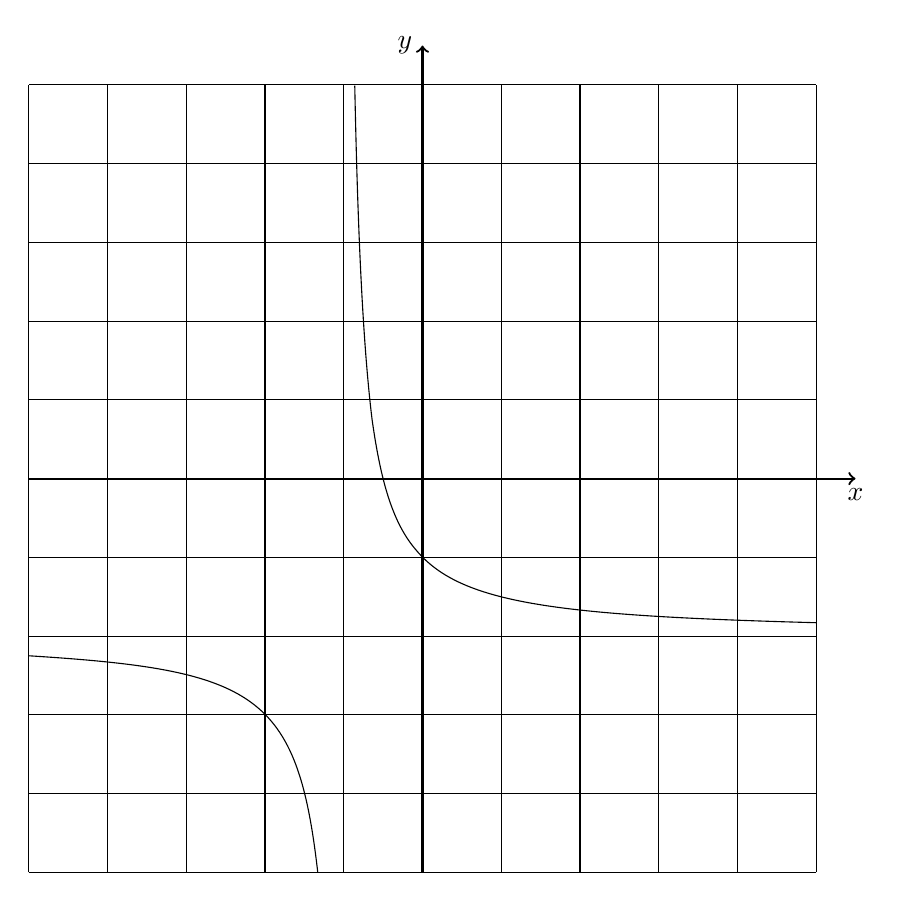
\begin{tikzpicture}
	\draw (-5,-5) grid (5,5);
	\draw[thick,->] (-5,0) -- (5.5,0) node[below]{$x$};
	\draw[thick,->] (0,-5) -- (0,5.5) node[left]{$y$};  
	\draw (-5,-2.25) .. controls (-2.12,-2.43) and (-1.59,-2.72) .. (-1.33,-5)
	(-0.86,4.99) .. controls (-0.82,3.01) and (-0.75,1.65) .. (-0.64,0.75) 
	.. controls (-0.53,-0.03) and (-0.38,-0.57) .. (-0.07,-0.92) 
	.. controls (0.5,-1.59) and (1.7,-1.74) .. (5,-1.83);
\end{tikzpicture}
\end{document}
\end{verbatim}
and you will get the following picture:
\begin{center}
	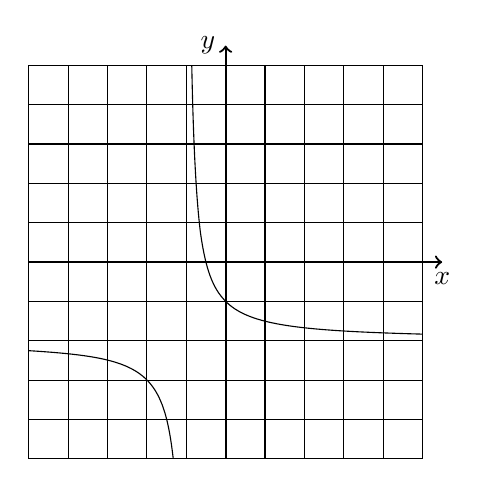
\begin{tikzpicture}[scale=.5]
		\draw (-5,-5) grid (5,5);
		\draw[thick,->] (-5,0) -- (5.5,0) node[below]{$x$};
		\draw[thick,->] (0,-5) -- (0,5.5) node[left]{$y$};  
		\draw (-5,-2.25) .. controls (-2.12,-2.43) and (-1.59,-2.72) .. (-1.33,-5)(-0.86,4.99) .. controls (-0.82,3.01) and (-0.75,1.65) 
	.. (-0.64,0.75) .. controls (-0.53,-0.03) and (-0.38,-0.57) .. (-0.07,-0.92) .. controls (0.5,-1.59) and (1.7,-1.74) .. (5,-1.83);
	\end{tikzpicture}
\end{center}
\section{Examples of \texttt{bezierplot} in Comparison with Gnuplot}
The following graphs are drawn with \texttt{bezierplot} (black) and Gnuplot (red). Gnuplot calculated 200 samples per example. The functions are given below the pictures (left: bezierplot, right: Gnuplot).
\begin{multicols}{3}
\graphcomparison{0.32*x-0.7}{0.32*x-0.7}
\graphcomparison{-x^2+4}{-x**2+4}
\graphcomparison{(x+1)*x*(x-1)}{(x+1)*x*(x-1)}
\graphcomparison{x^0.5}{x**0.5}
%\graphcomparison{x^(1/3)}{x**(1/3.)}
\graphcomparison{cbrt(x)}{sgn(x)*abs(x)**(1/3.)}
\graphcomparison{x^3*(x-1)}{x**3*(x-1)}
\graphcomparison{2*cos(3*x+4)+3}{2*cos(3*x+4)+3}
\graphcomparison{tan(x)}{tan(x)}
\graphcomparison{x+0.5*sin(x)}{x+0.5*sin(x)}
%\graphcomparison{1/(x-2)+1}{1/(x-2)+1}
\graphcomparison{2*x^2/(3*x-3)}{2*x**2/(3*x-3)}
\graphcomparison{4-exp(x)}{4-exp(x)}
\graphcomparison{log(x+4)}{log(x+4)}
\end{multicols}
\section{Are the Graphs Produced by bezierplot Exact?}
The graphs of quadratic and cubic functions and their inverse are exact (up to numeric precision). Sine and cosine functions use the predefined splines from Ti\emph{k}Z (which are very close approximations) if possible. E.g.
\begin{verbatim}
bezierplot "cos(x)"
\end{verbatim}
outputs
\begin{verbatim}
(-5,0.284) .. controls (-4.909,0.196) and (-4.818,0.105) .. (-4.713,0) 
sin (-3.142,-1) cos (-1.571,0) sin (0,1) cos (1.571,0) sin (3.142,-1) 
cos (4.713,0) .. controls (4.818,0.105) and (4.909,0.196) .. (5,0.284)
\end{verbatim}
\section{Options}
You can set the window of the graph as follows:
\begin{verbatim}
bezierplot "FUNCTION" XMIN XMAX YMIN YMAX
\end{verbatim}
e.g.
\begin{verbatim}
bezierplot "FUNCTION" 0 1 -3 2.5
\end{verbatim}
will set $0\leq x\leq 1$ and $-3\leq y\leq 2.5$. You may also omit the $y$--range, hence
\begin{verbatim}
bezierplot "FUNCTION" 0 1
\end{verbatim}
will set $0\leq x\leq 1$ and leave the default $-5\leq y\leq 5$.
\section{Daily Use with \LaTeX{} and Lua\LaTeX}
Supposing your OS finds \texttt{bezierplot} automatically (e.g. because it is in \verb|/usr/local/bin|), you can set up your \LaTeX{} file like this:
\begin{verbatim}
\documentclass{article}
\usepackage{tikz}
\makeatletter\let\evaluatedinput\@@input\makeatother
\providecommand{\bezierplot}[1]{\evaluatedinput|"bezierplot '#1'" }
\begin{document}
\tikz \draw \bezierplot{x^2};
\end{document}
\end{verbatim}
If you run \LaTeX{} with enabled shell-escape (option \verb|--shell-escape| for \TeX{}Live, option \verb|--write18| for MiK\TeX{}), you will receive automatically the following picture:
\begin{center}
	\begin{tikzpicture}[scale=.5]
		\draw \bezierplot{sqrt(x)};
	\end{tikzpicture}
\end{center}
Things get even better with Lua\LaTeX{}, because it can call Lua directly and do not need shell-escape enabled:
\begin{verbatim}
\documentclass{article}
\usepackage{tikz,xparse}
\directlua{require("bezierplot")}
\DeclareExpandableDocumentCommand{\xbezierplot}{O{-5} O{5} O{-5} O{5} m}{%
\directlua{tex.sprint(bezierplot("#5",#1,#2,#3,#4))}}
\providecommand\bezierplot{\romannumeral`\^^@\xbezierplot}
\begin{document}
\tikz \draw \bezierplot{x^2};
\end{document}
\end{verbatim}
The above example also extends the \verb|\bezierplot| command in such way, that you may set the bounds as options: E.g. \verb|\bezierplot[0][1][2]{x^2}| will set $0\leq x\leq 1$ and $2\leq y \leq 5$.
\end{document}
